\appendix
\chapter{Test de continuité}\label{cnt}
  
  La figure \ref{testcnt} présente une comparaison de différents calculs \EOS, notamment avec 
  l'interpolateur\footnote{Ce test est exécutable, avec la méthode \str{Thetis} au lieu de \str{Refprop} ici, via la commande \Cpp{EOSTestIpp},
  développé dans le fichier: \str{version}/Modules/EOS/Tests/C++/main\_ipp.cxx}.
  Le but de ces courbes est de montrer l'efficacité de l'algorithme de continuité et d'assurer ainsi l'homogénéité des propriétés physiques dans tout le maillage.
  Le maillage a été créé à l'aide de la méthode Refprop d'\EOS\ et le raffinement est imposé 
  par un critère de qualité ayant comme propriété la Température.
  Le Test est réalisé pour la propriété \textbf{cp}, à \textbf{h} constant $ h=2,87 \cdot 10^{6} J$ et 
  \textbf{p} variant de $ 1,3 \cdot 10^{5} Pa$ à $ 2,0 \cdot 10^{5} Pa$ avec un grand nombre de points:
  \begin{figure}[H]
    \center
    \includegraphics[width=1\textwidth]{Cp_continuite.eps}
    \caption{Test de continuité.}\label{testcnt}
  \end{figure}
  \textbf{Détail du graphique:}
  \smallbreak\vspace{0.3cm}
  Les mailles 1 et 2 ne sont pas raffinées, les mailles 3 et 4 proviennent de la même maille raffinée.
  \vspace{0.3cm}
  \begin{itemize}
   \item[\textbullet] La courbe en pointillés vert utilise la méthode \textbf{Refprop} d'\EOS\ et représente la référence.
   \vspace{0.2cm}
   \item[\textbullet] La courbe noire a été effectuée grâce à l'interpolateur et un maillage sans raffinement, 
   ce qui fait qu'il n'y a aucune correction permettant de se rapprocher de la référence.
   \vspace{0.2cm}
   \item[\textbullet] La courbe bleue a été réalisée avec l'interpolateur et une \bdd, dont la création n'utilise pas l'algorithme de continuité.
   Cette courbe montre bien qu'à la frontière des mailles 2 et 3 la propriété \textbf{cp} n'est pas continue.
   \vspace{0.2cm}
   \item[\textbullet] La courbe rouge, au contraire, a été tracée à l'aide d'une \bdd\ continue, ce qui induit une meilleure interpolation dans la maille 2.
   Il est remarquable, que cette courbe possède un coude dans la maille 2, ceci est dû à une continuité croisée (Cf. Figure \ref{2cont}).
  \end{itemize}

  
  
  
  
 
 
  
